\section{Computer Setup}
\begin{information}
We will all be working on our own computers today, and will be accessing Virtual Machines running the Ubuntu operating system on \texttt{phoenix}, which is the University of Adelaide's High Performance Computing (HPC) system.
The software client \texttt{X2GO} which you will have already installed, enables us to access these machines in a familiar Desktop style, even though the majority of our time will be spent within the terminal. \\
\end{information}

You will have been allocated a VM with an associated IP address.
To connect to your VM, \textbf{please follow these instructions carefully}.
First, we need to create a session with the basic parameters
\begin{enumerate}
	\item Open X2GO
	\item Enter \textit{IntroductionToBash} as the \textbf{Session Name}
	\item Enter your \textit{IP address} where it say \textbf{Host}
	\item Enter the word \textbf{hub} as the login. \textbf{This must be all lower-case}
	\item Select \textbf{XFCE} from the drop-down menu under \textbf{Session Type}
	\item Click OK
\end{enumerate}

Now we have created the session, it will appear in your X2Go on the right.
To log onto the VM, we simply click on the session, and enter the password \textbf{hub}.
\textbf{Click OK if you receive a message about a security key}.
If this process fails, please place the red post-it note on your monitor.\\

\textit{We advise maximising your X2Go window to replicate sitting at the VM as if it is your local machine.}

\begin{figure}[ht]
	\centering
	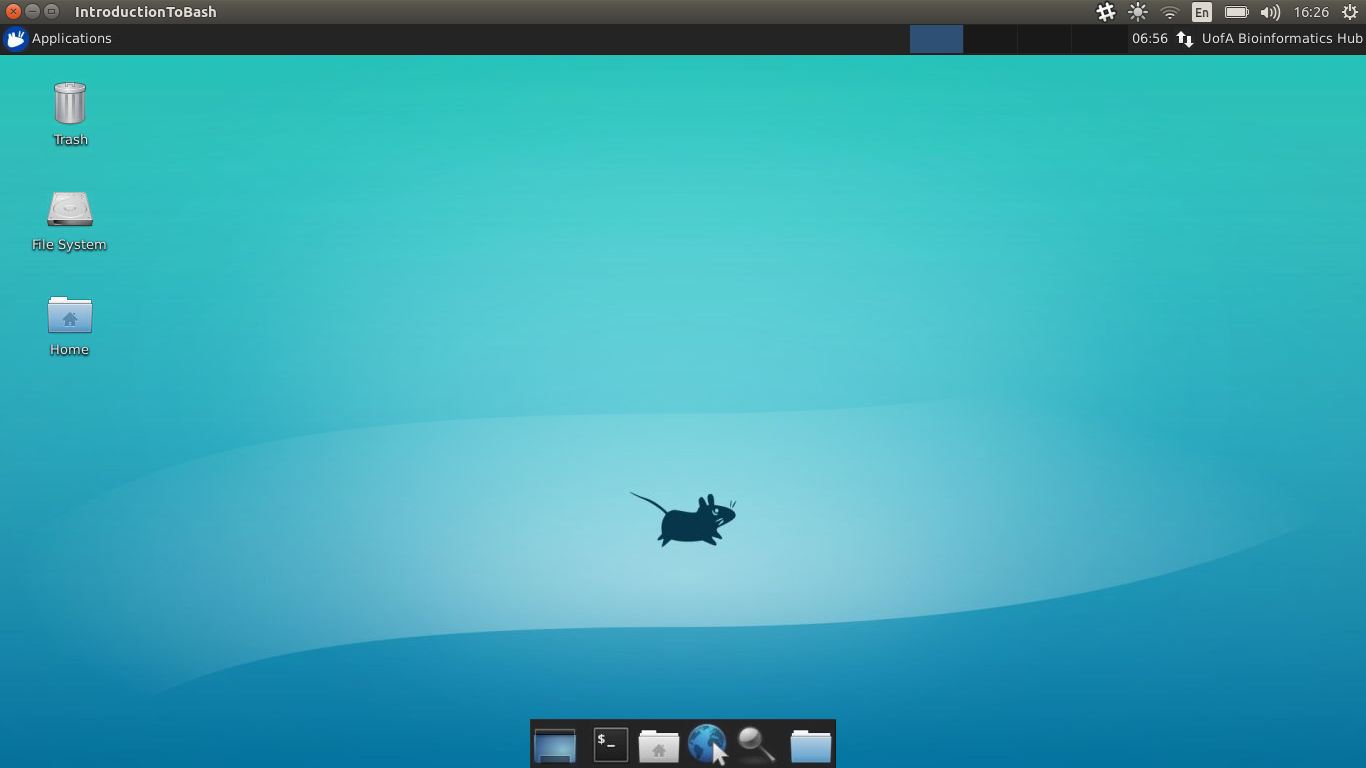
\includegraphics[width=0.9\linewidth]{images/xfceDesktop.png} 
	\caption{The VM desktop after logon with X2GO}
\end{figure}


\section{The Ubuntu Desktop}
\begin{note}
Now that you are connected, you will notice we are in a standard graphical environment.
The default Desktop in Ubuntu is Unity, but what we are seeing is one of the many alternatives, known as XFCE.
We are using this as it is the most simple for remote connections.
As many of us are used to seeing, there are click-able icons on the desktop, and drop-down menus. \\

Although we won't be using them today, Ubuntu has an built-in Office Suite of
programs which you can access from the \textit{Applications \textgreater Office} menu item.
This is where links can be found to open Document Viewer (a .pdf viewer), Libre Office Calc (Excel-like), Libre Office Writer (Word-like) \& other standard members of Office Program Suites. \\

The main interface we will be using today is the \texttt{terminal}which can be accessed from the set of icons at the bottom of you screen.
\textbf{Firefox} can also be accessed from the terminal using the command \texttt{firefox \&},  by clicking the \texttt{Web Browser} icon, or from the drop-down menu in the top left under the group \textit{Internet}.

\end{note}

